\documentclass{beamer}

\mode<presentation>
{
  \usetheme{Madrid}
  % or ...
  \setbeamertemplate{bibliography item}{}
  \setbeamercovered{transparent}
  % or whatever (possibly just delete it)
}

\usepackage{fontspec}
\usepackage[english]{babel}
% or whatever
\usepackage{csquotes}
\usepackage[backend=biber,
        style=unified,
        maxcitenames=3,
        maxbibnames=99,
        natbib,
        url=false]{biblatex}
\addbibresource{Dissertation.bib}
\setmainfont{Linux Libertine O}
\setmonofont{CMU Typewriter Text}
\renewcommand{\ttdefault}{cmtt}

% \usepackage[colorlinks,allcolors={black},urlcolor={blue}]{hyperref} %allows for hyperlinks and pdf bookmarks 
\usepackage{graphicx}	%Inserting graphics, pictures, images 		
\usepackage{multicol} %Multicolumn text
\usepackage{multirow} %Useful for combining cells in tablesbrew 
\usepackage{booktabs} %Enhanced tables
% \usepackage{underscore} %Allows for underscores in text mode
% \usepackage[colorlinks,allcolors={black},urlcolor={blue}]{hyperref} %allows for hyperlinks and pdf bookmarks
\usepackage{url} %allows for urls
\def\UrlBreaks{\do\/\do-} %allows for urls to be broken up
% \usepackage[normalem]{ulem} %strike out text. Handy for syntax
% \usepackage{tcolorbox}
% \usepackage{datetime2}
% \usepackage{caption}
% \usepackage{subcaption}
\usepackage{tipa} %IPA symbols
% \usepackage[documentfont=DoulosSIL]{tipauni}
\usepackage{langsci-gb4e} % Language Science Press' modification of gb4e
\usepackage{tikz} % Drawing Hasse diagrams
\usetikzlibrary{decorations.pathreplacing}
\usepackage{leipzig} %	Offers support for Leipzig Glossing Rules

%%MACROS
\newcommand{\sub}[1]{\textsubscript{#1}}
\newcommand{\supr}[1]{\textsuperscript{#1}}
\providecommand{\lsptoprule}{\midrule\toprule}
\providecommand{\lspbottomrule}{\bottomrule\midrule}
\newcommand{\fittable}[1]{\resizebox{\textwidth}{!}{#1}}


\title[Voice Quality in SLZ] % (optional, use only with long paper titles)
{Voice Quality and Laryngeal Complexity in Santiago Laxopa Zapotec}

% \subtitle{Include Only If Paper Has a Subtitle}

\author[Brinkerhoff] % (optional, use only with lots of authors)
{Mykel Loren Brinkerhoff}
% - Give the names in the same order as the appear in the paper.
% - Use the \inst{?} command only if the authors have different
%   affiliation.

\institute[UC Santa Cruz] % (optional, but mostly needed)
{University of California, Santa Cruz}
% - Use the \inst command only if there are several affiliations.
% - Keep it simple, no one is interested in your street address.

\date[2025-06-06] % (optional, should be abbreviation of conference name)
{6 June 2025}
% - Either use conference name or its abbreviation.
% - Not really informative to the audience, more for people (including
%   yourself) who are reading the slides online

% \subject{Theoretical Computer Science}
% This is only inserted into the PDF information catalog. Can be left
% out. 



% If you have a file called "university-logo-filename.xxx", where xxx
% is a graphic format that can be processed by latex or pdflatex,
% resp., then you can add a logo as follows:

\pgfdeclareimage[height=0.5cm]{university-logo}{images/UCSC_Logo_RGB.png}
\logo{\pgfuseimage{university-logo}}



% Delete this, if you do not want the table of contents to pop up at
% the beginning of each subsection:
% \AtBeginSubsection[]
% {
%   \begin{frame}<beamer>{Outline}
%     \tableofcontents[currentsection,currentsubsection]
%   \end{frame}
% }


% If you wish to uncover everything in a step-wise fashion, uncomment
% the following command: 

%\beamerdefaultoverlayspecification{<+->}


\begin{document}

\begin{frame}
  \titlepage
\end{frame}

\begin{frame}{Outline}
  \tableofcontents
  % You might wish to add the option [pausesections]
\end{frame}


% Structuring a talk is a difficult task and the following structure
% may not be suitable. Here are some rules that apply for this
% solution: 

% - Exactly two or three sections (other than the summary).
% - At *most* three subsections per section.
% - Talk about 30s to 2min per frame. So there should be between about
%   15 and 30 frames, all told.

% - A conference audience is likely to know very little of what you
%   are going to talk about. So *simplify*!
% - In a 20min talk, getting the main ideas across is hard
%   enough. Leave out details, even if it means being less precise than
%   you think necessary.
% - If you omit details that are vital to the proof/implementation,
%   just say so once. Everybody will be happy with that.
%-----------------------------------------------------------
\section{Introduction}
%-----------------------------------------------------------
%-----------------------------------------------------------
\subsection{Overview of my dissertation}
%-----------------------------------------------------------

\begin{frame}{Research Overview}
  \begin{itemize}
    \item What my research is about:
  \end{itemize}
\end{frame}

\begin{frame}{Research Questions}
  \begin{block}{Questions:}
    \begin{itemize}
      \item How is phonation's acoustic space structured in a single language?
      \item Which measures are important for capturing phonation contrasts?
      \item How do these measures help explain SLZ's laryngeal complexity?
    \end{itemize}
  \end{block}
\end{frame}

\begin{frame}{Research Questions}
  \begin{block}{Answers:}
    \begin{itemize}
      \item Yes; we find a three-dimensional space.
      \item Dimensions in Santiago Laxopa Zapotec are correlated with:
      \begin{enumerate}
        \item First/third dimension $=$ glottal-airflow continuum. 
        \item Second dimension $=$ nonmodal-to-modal continuum.
      \end{enumerate}
    \end{itemize}  
  \end{block}
\end{frame}

%-----------------------------------------------------------
\subsection{What is Voice Quality?}
%-----------------------------------------------------------

\begin{frame}{What is Voice Quality?}
  \begin{itemize}
  \item
    Describes how the vocal folds vibrate.
  \item
    Used for both paralinguistic \citep[e.g.,][]{laverVoiceQualityIndexical1968,podesvaStanceWindowLanguageRace2016} and phonological contrasts \citep[e.g.,][]{espositoCrosslinguisticPatternsPhonation2020}.
  \end{itemize}
\end{frame}

\begin{frame}{How is voice quality used?}
  \begin{itemize}
    \item Voice quality is a complex phenomenon that is not fully understood.
    \item It is often described in terms of phonation types, such as:
    \begin{itemize}
      \item Modal
      \item Breathy
      \item Creaky
      \item Whispery
    \end{itemize}
  \end{itemize}
\end{frame}

%-----------------------------------------------------------
\subsection{Santiago Laxopa Zapotec}
%-----------------------------------------------------------

\begin{frame}{Santiago Laxopa Zapotec}
  \begin{columns}
    \begin{column}{0.33\textwidth}
      \begin{itemize}
        \item Santiago Laxopa Zapotec (SLZ; \textit{Dille'xhunh Laxup}) is a Sierra Norte variety of Zapotec.
        \item Spoken by c. 1,000 speakers in Santiago Laxopa and in diaspora.
      \end{itemize}
    \end{column}
    \begin{column}{0.67\textwidth}
      \begin{figure}
        \centering
        \includegraphics[width=0.95\linewidth]{images/Oaxaca_Santiago_Laxopa_Map.eps}
      \end{figure}
    \end{column}
  \end{columns}
\end{frame}

\begin{frame}{Phonation in SLZ}
  \begin{itemize}
    \item SLZ has a four-way phonation contrast:
    \begin{itemize}
      \item Modal ( [\textipa{a}] )
      \item Breathy ( [\textipa{\"*a}] )
      \item Checked ( [\textipa{\t{aP}}] or [\textipa{\t{a\~*a}}] )
      \item Rearticulated ([\textipa{\t{aPa}}], [\textipa{\t{a\~*aa}}], or [\textipa{\~*a}] )
    \end{itemize}
    \item SLZ's phonation contrasts are used in both the phonology and the morphology.
  \end{itemize}
\end{frame}

\begin{frame}{Tone in SLZ}
  \begin{itemize}
    \item 
  \end{itemize}
\end{frame}

\begin{frame}{Interaction of Tone and Phonation in SLZ}
  \begin{itemize}
    \item 
  \end{itemize}
  
\end{frame}

%-----------------------------------------------------------
\section{Previous research}
%-----------------------------------------------------------
%-----------------------------------------------------------
\subsection{Measuring Voice Quality}
%-----------------------------------------------------------

\begin{frame}{Measuring voice quality}
  \begin{itemize}
    \item Long been established that phonation has correlates in the acoustic signal (e.g., \cite{fischer-jorgensenPhoneticAnalysisBreathy1968,klattAnalysisSynthesisPerception1990}).
    \item \citet{gordonPhonationTypesCrosslinguistic2001} list several types of measures types that can be used:
    \begin{itemize}
    \item Periodicity
    \item Energy
    \item Spectral tilt
    \item Pitch
    \item Duration 
    \end{itemize}
  \item Linguists have used combinations of these measures to model phonation (e.g., \cite{blankenshipTimingNonmodalPhonation2002,brunelleTonePhonationSoutheast2016,espositoAcousticElectroglottographicStudy2012}). 
  \end{itemize}
\end{frame}

\begin{frame}{New measures of voice quality}
  
\end{frame}

\begin{frame}{Too many measures}
  
\end{frame}

%-----------------------------------------------------------
\subsection{Modeling Voice Quality}
%-----------------------------------------------------------


\begin{frame}{Modeling voice quality}
  \begin{itemize}
    \item Early models proposed that voice quality is one dimensional and represents glottal airflow \citep{ladefogedPreliminariesLinguisticPhonetics1971,ladefogedSoundsWorldsLanguages1996}.
  \end{itemize}
  \begin{figure}[h!]
    % \centering
    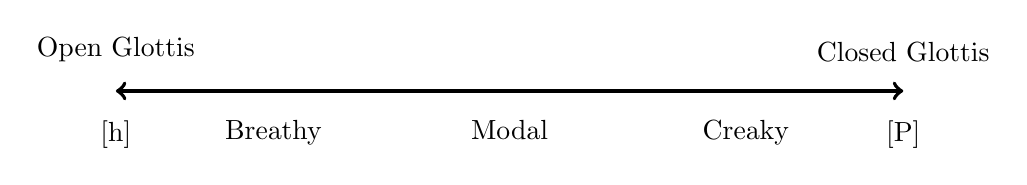
\begin{tikzpicture}
        % Draw the line with arrows at both ends
        \draw[<->, line width=0.5mm] (0,0) -- (10,0);
        
        % Labels underneath the line
        \node[below, yshift=-0.25cm] at (0,0) {[\textipa{h}]};
        \node[below, yshift=-0.25cm] at (2,0) {Breathy};
        \node[below, yshift=-0.25cm] at (5,0) {Modal};
        \node[below, yshift=-0.25cm] at (8,0) {Creaky};
        \node[below, yshift=-0.25cm] at (10,0) {[\textipa{P}]};
        
        % Labels above the line
        \node[above, yshift=0.25cm] at (0,0) {Open Glottis};
        \node[above, yshift=0.25cm] at (10,0) {Closed Glottis};
    \end{tikzpicture}
    % \caption{A diagram showing the relationship between breathy, modal, and creaky phonation types from \citet{gordonPhonationTypesCrosslinguistic2001}.}
    % \label{fig:phonation_types}
\end{figure}
\end{frame}

\begin{frame}{Voice quality's multidimensionality}
  \begin{itemize}
    \item More recent work has shown that voice quality is not one-dimensional, but minimally five-dimensional \citep[e.g.,][]{garellekModelingVoiceSource2016,kreimanValidatingPsychoacousticModel2021}.
    \begin{itemize}
      \item Especially in the case of individual speaker differences.
    \end{itemize}
    \item \citet{garellekVoiceQualityTone2013} has argued that dimensionality might not be as complex for capturing phonation contrasts.
  \end{itemize}
\end{frame}

\begin{frame}{\citet{keatingCrosslanguageAcousticSpace2023}}
  \begin{itemize}
    \item Explored phonation's cross-linguistic acoustic space.
    \item Found a two-dimensional space for phonation across 11 languages.
    \begin{enumerate}
      \item First dimension $=$ nonmodal-to-modal continuum.
      \item Second dimension $=$ glottal-airflow continuum.
    \end{enumerate}
    \item Found that languages with more contrasts used more of the acoustic space than languages with fewer contrasts.
    \item Found correlations between dimensions and acoustic measures.
    \begin{enumerate}
      \item First dimension $=$ periodicity and energy.
      \item Second dimension $=$ spectral tilt and periodicity.
    \end{enumerate}
  \end{itemize}
\end{frame}

\begin{frame}{\citet{keatingCrosslanguageAcousticSpace2023}}
  \begin{figure}[h!]
    \centering
    \includegraphics[width = 0.8\linewidth]{images/Keating_dimension.png}
  \end{figure}
\end{frame}

%-----------------------------------------------------------
\subsection{Laryngeal Complexity}
%-----------------------------------------------------------

\begin{frame}{What is Laryngeal Complexity}
  \begin{itemize}
    \item Laryngeal complexity is the number of phonation contrasts in a language.
    \item More phonation contrasts means more complex laryngeal system.
    \item Laryngeal complexity can be measured by the number of phonation contrasts in a language.
    \item Laryngeal complexity can be measured by the dimensionality of the acoustic space.
  \end{itemize}
\end{frame}

\begin{frame}{Phonation's phasing}
  
\end{frame}

\begin{frame}{Implicational hierarchy of patterns}
  
\end{frame}

\begin{frame}{Previous research on laryngeal complexity}

\end{frame}

%-----------------------------------------------------------
\section{My Results}
%-----------------------------------------------------------
%-----------------------------------------------------------
\subsection{Data and Methods}
%-----------------------------------------------------------
\begin{frame}{Data}
  \begin{itemize}
    \item Data comes from fieldwork on Santiago Laxopa Zapotec (SLZ) from Summer 2023.
    \item Production data was collected from 10 speakers (5 male/5 female).
  \end{itemize}
\end{frame}

%-----------------------------------------------------------
\subsection{Acoustic Landscape}
%-----------------------------------------------------------

\begin{frame}{MDS analysis}
  \begin{itemize}
    \item Multidimensional scaling (MDS; \cite{kruskalMultidimensionalScaling1978}) was used to reduce the dimensionality of the data.
    \item Acoustic measures used to define the acoustic space, following \citet{keatingCrosslanguageAcousticSpace2023}.
    \item Speaker x phonation combinations were used for the points in the MDS space.
  \end{itemize}
\end{frame}

\begin{frame}{Number of Dimensions}
  \begin{figure}[h!]
    \centering
    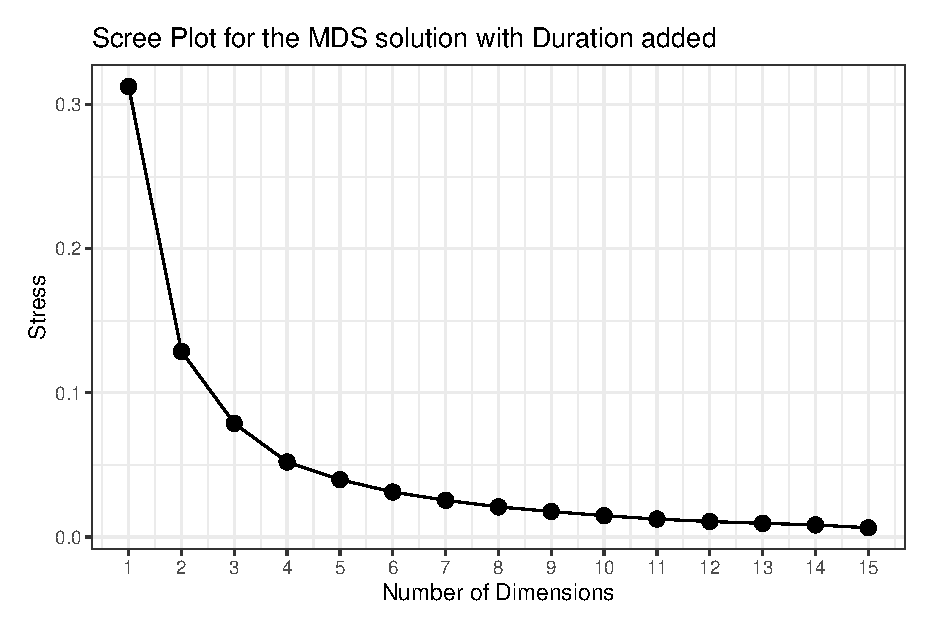
\includegraphics[width = 0.8\linewidth]{images/MDS/stress_plot_dur.eps}
\end{figure}
\end{frame}

\begin{frame}{Dimensionality in SLZ}
  \begin{itemize}
    \item Scan the QR code to see the three-dimensional space.
  \end{itemize}
  \begin{figure}[h!]
    \centering
    \includegraphics[width=5cm, scale=0.5]{qrcode_3d_plot.eps}
  \end{figure}
\end{frame}

\begin{frame}{Dimensionality in SLZ}
  \begin{figure}
    \centering
    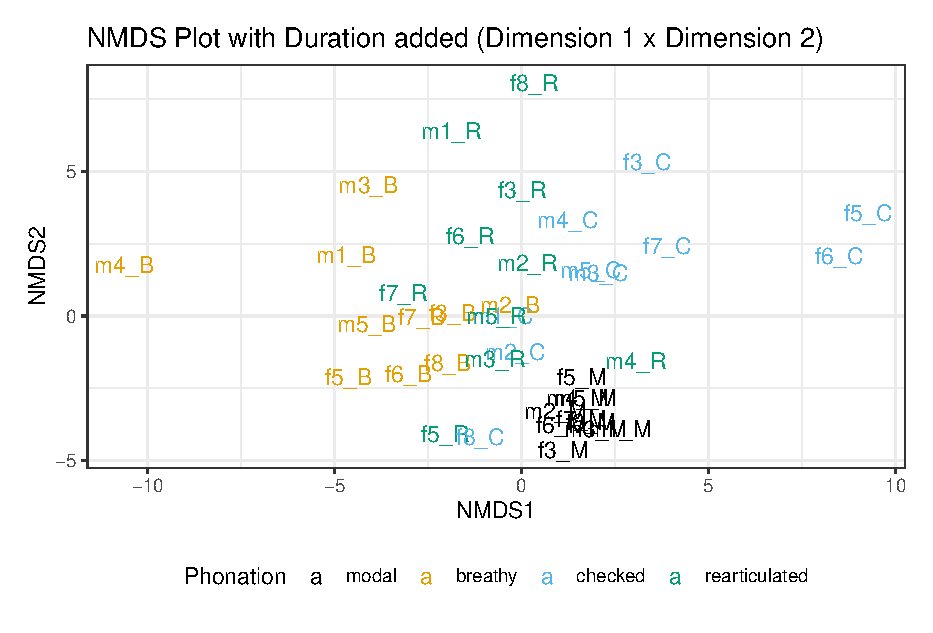
\includegraphics[width = 0.8\linewidth]{images/MDS/nmds12_dur.eps}
  \end{figure}
\end{frame}

\begin{frame}{Dimensionality in SLZ}
  \begin{figure}
    \centering
    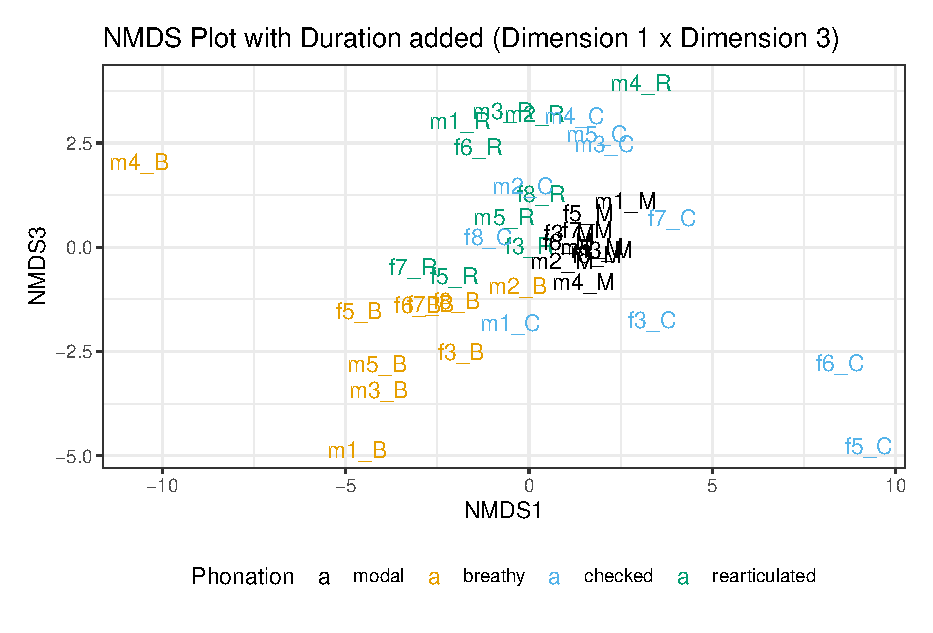
\includegraphics[width = 0.8\linewidth]{images/MDS/nmds13_dur.eps}
  \end{figure}
\end{frame}

\begin{frame}{Dimensionality in SLZ}
  \begin{figure}
    \centering
    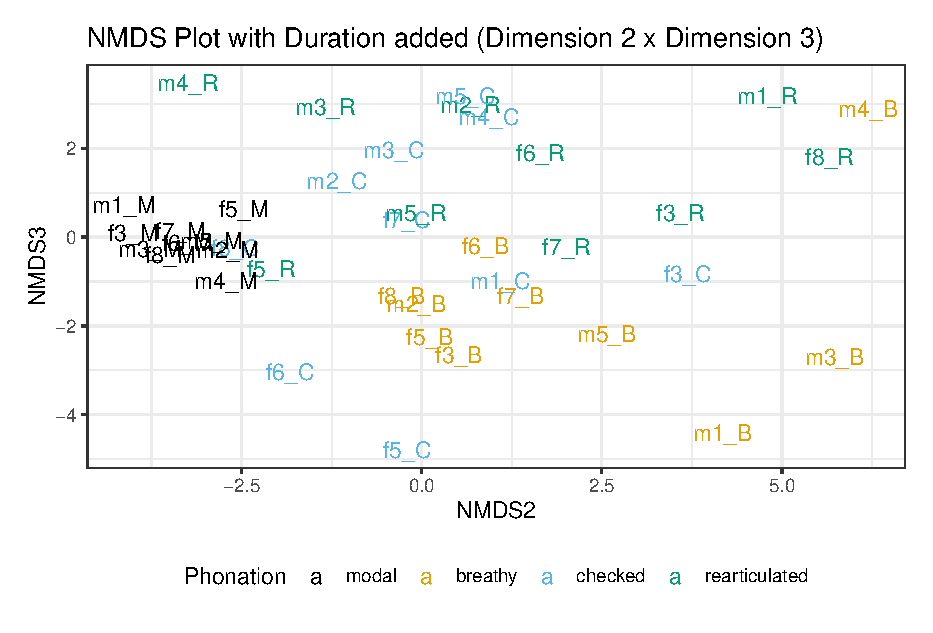
\includegraphics[width = 0.8\linewidth]{images/MDS/nmds23_dur.eps}
  \end{figure}
\end{frame}

\begin{frame}{Summary of Dimensions}
  \begin{itemize}
    \item Dimension 1 (D1) gives a rough continuum from breathy to creaky.
    \item Dimension 2 (D2) gives a rough continuum from modal to nonmodal.
    \item Dimension 3 (D3) gives a rough continuum from breathy to creaky.
  \end{itemize}
\end{frame}

\begin{frame}{Correlation to Acoustic Measures}
  \begin{itemize}
    \item D1 correlated with spectral tilt measures: 
    \begin{itemize}
      \item H1*$-$A1* ($r^2 = -0.83$) 
      \item H1*$-$A2* ($r^2 = -0.86$)
      \item H1*$-$A3* ($r^2 = -0.81$)
    \end{itemize}
    \item D2 correlated with periodicity and energy: 
    \begin{itemize}
      \item HNR\textless 500 Hz ($r^2 = -0.79$)
      \item HNR\textless 1500 Hz ($r^2 = -0.80$)
      \item Energy ($r^2 = -0.79$)
    \end{itemize}
    \item D3 correlated with spectral tilt:
    \begin{itemize}
      \item residual H1* ($r^2 = -0.72$)
      \item H2*$-$H4* ($r^2 = -0.69$)
      \item H2* ($r^2 = -0.68$)
    \end{itemize}
  \end{itemize}
\end{frame}

\begin{frame}{Summary of Acoustic Landscape}
  \begin{itemize}
    \item SLZ's phonation occupies a three-dimensional space.
    \item Dimensions are correlated with glottal-airflow continuum (D1/D3) and nonmodal-to-modal continuum (D2).
    \item Dimensions are similar to those found in \citet{keatingCrosslanguageAcousticSpace2023}.
  \end{itemize}
\end{frame}

%-----------------------------------------------------------
\subsection{Random Forests}
%-----------------------------------------------------------

\begin{frame}{What is Random Forest?}
  
\end{frame}

\begin{frame}{Results of Random Forest}
  
\end{frame}

\begin{frame}
  \frametitle{Variable Importance}
  \begin{figure}[h!]
    \centering
    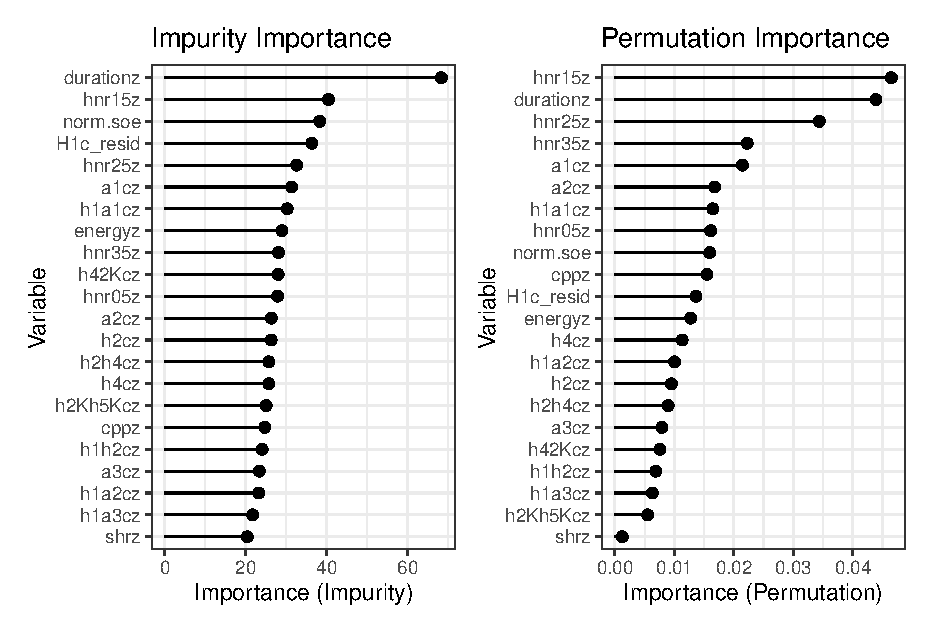
\includegraphics[width = 0.8\linewidth]{images/RandomForest/rf_dur_plots.eps}
  \end{figure}
\end{frame}

\begin{frame}{Summary of Random Forest}
  
\end{frame}

%-----------------------------------------------------------
\subsection{Laryngeal Complexity in SLZ}
%-----------------------------------------------------------

\begin{frame}{Generalized Additive Models (GAMs)}
  \begin{itemize}
    \item Used to explore the relationship between phonation and the acoustic measures.
    \item Used to explore the relationship between phonation and the MDS dimensions.
    \item Used to explore the relationship between phonation and the random forest dimensions.
  \end{itemize}
\end{frame}

\begin{frame}{Measuring Laryngeal Complexity}
  \begin{itemize}
    \item Laryngeal complexity is measured by the number of phonation contrasts in a language.
    \item SLZ has four phonation contrasts.
    \item The more phonation contrasts a language has, the more complex its laryngeal system is.
  \end{itemize}
\end{frame}

\begin{frame}{Summary of Laryngeal Complexity}
  \begin{itemize}
    \item SLZ has four phonation contrasts.
    \item SLZ's phonation occupies a three-dimensional space.
    \item Dimensions are correlated with glottal-airflow continuum (D1/D3) and nonmodal-to-modal continuum (D2).
    \item Dimensions are similar to those found in \citet{keatingCrosslanguageAcousticSpace2023}.
  \end{itemize}
\end{frame}

%-----------------------------------------------------------
\section{Summary and conclusions}
%-----------------------------------------------------------
\begin{frame}{Summary of Results}
  \begin{itemize}
    \item SLZ's phonation occupies a three-dimensional space.
    \item Dimensions are correlated with glottal-airflow continuum (D1/D3) and nonmodal-to-modal continuum (D2).
    \begin{itemize}
      \item Collaborated with acoustic measure correlations.
    \end{itemize}
    \item Dimensions are similar to those found in \citeauthor{keatingCrosslanguageAcousticSpace2023}.
  \end{itemize}
\end{frame}

\begin{frame}{Summary}
  \begin{itemize}
    \item Acoustic space can be reduced to two dimensions.
    \item More dimensions add more information about these two dimensions.
  \end{itemize}
  \begin{figure}[h!]
    \centering
    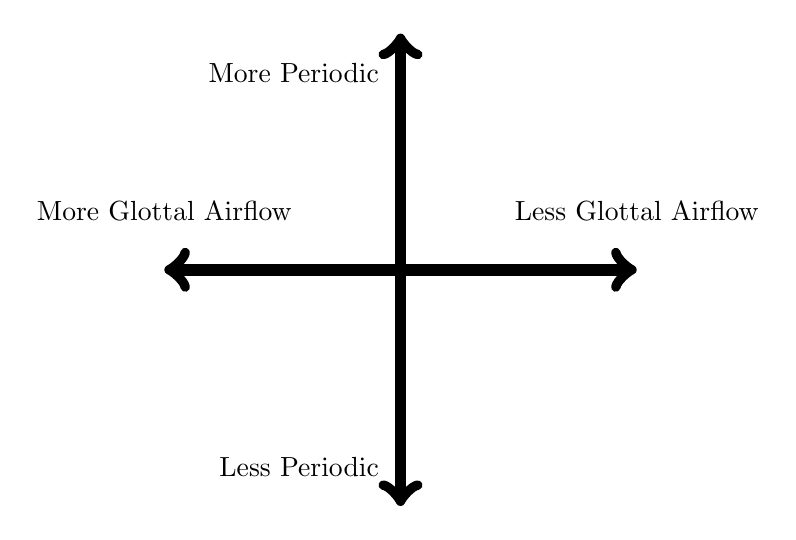
\begin{tikzpicture}
        % Draw the horizontal line with arrows
        \draw[<->, line width=1.5mm] (-3,0) -- (3,0);
        % Draw the vertical line with arrows
        \draw[<->, line width=1.5mm] (0,-3) -- (0,3);
        
        % Labels for the horizontal line
        \node[below,yshift=1cm] at (-3,0) {More Glottal Airflow};
        \node[below,yshift=1cm] at (3,0) {Less Glottal Airflow};
        
        % Labels for the vertical line
        \node[left, xshift = -1.5mm] at (0,-2.5) {Less Periodic};
        \node[left, xshift = -1.5mm] at (0,2.5) {More Periodic};
    \end{tikzpicture}
\end{figure}
\end{frame}

\begin{frame}{Summary}

  % Keep the summary *very short*.
  \begin{itemize}
  \item Dimensionality reduction also occurs in a single language.
  \item Dimensions correspond to glottal-airflow and nonmodal-to-modal continua within a language and cross-linguistically.
  \item If additional dimensions are added, they only add additional information about these two dimension.
  \end{itemize}
  
  % The following outlook is optional.
  \vskip0pt plus.5fill
  \begin{itemize}
  \item
    Outlook
    \begin{itemize}
    \item What are the perceptual cues that speakers use to distinguish between phonation types?
    \item How do these dimensions relate to the phonology?
    \end{itemize}
  \end{itemize}
\end{frame}

\begin{frame}
  \frametitle{Duxhklhenhu' lhe' (Thank you)}
  \begin{figure}[h!]
    \centering
    \includegraphics[width = \linewidth]{images/SantiagoLaxopa.jpeg}
  %   \label{fig:fieldwork}
  \end{figure}
\end{frame}

%-----------------------------------------------------------
\section*{Acknowledgements}
%-----------------------------------------------------------

\begin{frame}
  \frametitle{Acknowledgements}
  \begin{itemize}
    \item Thank you to the speakers in Santiago Laxopa for sharing their time and language expertise. 
    \item Thank you to Grant McGuire, Jaye Padgett, Marc Garellek, Ryan Bennett, Jack Duff, Maya Wax Cavallaro, and many others for their help and discussions during all stages of this project. 
  \end{itemize}
\end{frame}

\begin{frame}
  \frametitle{Acknowledgements}
  This work is supported by funding from: 
  \begin{itemize}
    \item The National Science Foundation under Grant No. 2019804
    \item The Humanities Institute at UC Santa Cruz 
    \item The Jacobs Research Funds
  \end{itemize}

\end{frame}


\appendix
%-----------------------------------------------------------
\section<presentation>*{\appendixname}
%-----------------------------------------------------------
%-----------------------------------------------------------
\section{References}
%-----------------------------------------------------------
\begin{frame}[t,allowframebreaks]
  \frametitle{References}
    \printbibliography
\end{frame}

\end{document}